%% PNAStwoS.tex
%% Sample file to use for PNAS articles prepared in LaTeX
%% For two column PNAS articles
%% Version: Apr 15, 2008 
 

%% BASIC CLASS FILE
\documentclass{pnastwo}


%% ADDITIONAL OPTIONAL STYLE FILES
%\usepackage[dvips]{graphicx}
%\usepackage{pnastwof}
\usepackage{amssymb,amsfonts,amsmath}
\usepackage[utf8]{inputenc}
\usepackage[activeacute, spanish]{babel}
\usepackage[dvips]{graphicx}
\selectlanguage{spanish}


%% OPTIONAL MACRO DEFINITIONS
\def\s{\sigma}


%%%%%%%%%%%%
%% For PNAS Only:
\url{www.pnas.org/cgi/doi/10.1073/pnas.0709640104}
\copyrightyear{2008}
\issuedate{Issue Date}
\volume{Volume}
\issuenumber{Issue Number}
%\setcounter{page}{2687} %Set page number here if desired
%%%%%%%%%%%%

\begin{document}

\title{An analysis of Lenin's work: Revolution, war, and fruta}

\author{Leonardo Lázzaro,\affil{1}{Universidad de Buenos Aires, Buenos Aires, Argentina},
Julián Peller,\affil{1}{Universidad de Buenos Aires, Buenos Aires, Argentina},
Juan Manuel Pérez,\affil{1}{Universidad de Buenos Aires, Buenos Aires, Argentina},
}

\contributor{Submitted to Proceedings of the National Academy of Sciences
of the United States of America}

\maketitle

\begin{article}
\begin{abstract}
In order to discover how much related were Lenin Works to Russian History in nearly 20th century, we use the information value concept to extract the most important words from them. Therefore, we find out how far are them from certain concepts such as
war, revolution, theory, etc. We expected this concepts to be nearer and farther to concepts 
treated in Lenin's works depending on the events ranging from 1900 to 1924.
\end{abstract}

\keywords{information value | natural language processing | lenin }

\abbreviations{NLP}

\section{Introduction}

\dropcap{I}n this article we study distances in metric spaces consisting on words, and how we can
represent a text (an ordered set of words) as a smaller subset of their most representative words.

In \cite{DARWIN}, Zanette and Montemurro defined the information value of a word in a text. This is
a real value that quantifies how much information that word carries according to the text. Let $T$ be a 
text, and $T'$ a random shuffled version of $T$, and $w$ a word appearing in $T$. 
By $S_T(w)$ we denote the Shannon Entropy of $w$ with respect to $T$ (See appendix for more info). 

The information value of $w$ in $T$ is 

\begin{equation}
  IV_T(w) = f_w* | S_T(w) - S_{T'}(w) | 
\end{equation}

where $f_w$ is the frequency of appearance of $w$ in $T$. This value captures, in some way, whether a word
has a distribution in text that is not exactly uniform; an order of the word in the text that brings some sense to it.

Having these value, we can pull the most representative words out of a text by selecting those of greater information value.

\section{Method}
\subsection{Text Corpus}
We gathered Lenin's work from the "Marxists Internet Archive". This proved to be a difficult task as the works were not in a common HTML format. The tool we used to do this is Scrapy, a very comprehensive Python crawling framework.

In order to reduce noise in the corpus, we filtered all the letters and works that were comparatively little. Our information value theory doesn't work very well with texts with little repetition of words, so we decided to remove texts with less than 2000 words. 

\begin{figure}
\centerline{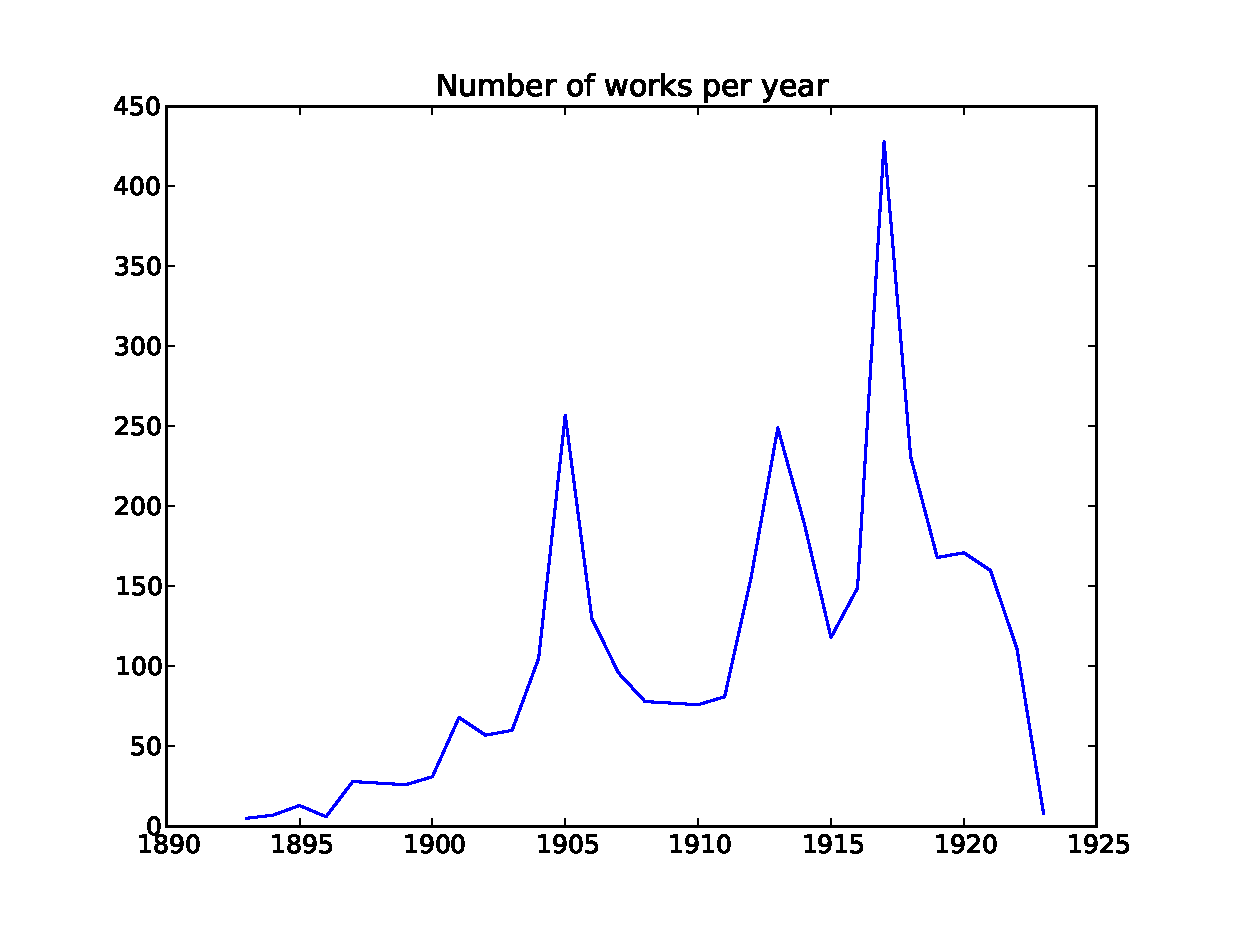
\includegraphics[width=.4\textwidth]{figures/tokens_per_year.eps}}
\caption{Number of works per year}\label{afoto}
\end{figure}

\begin{figure}
\centerline{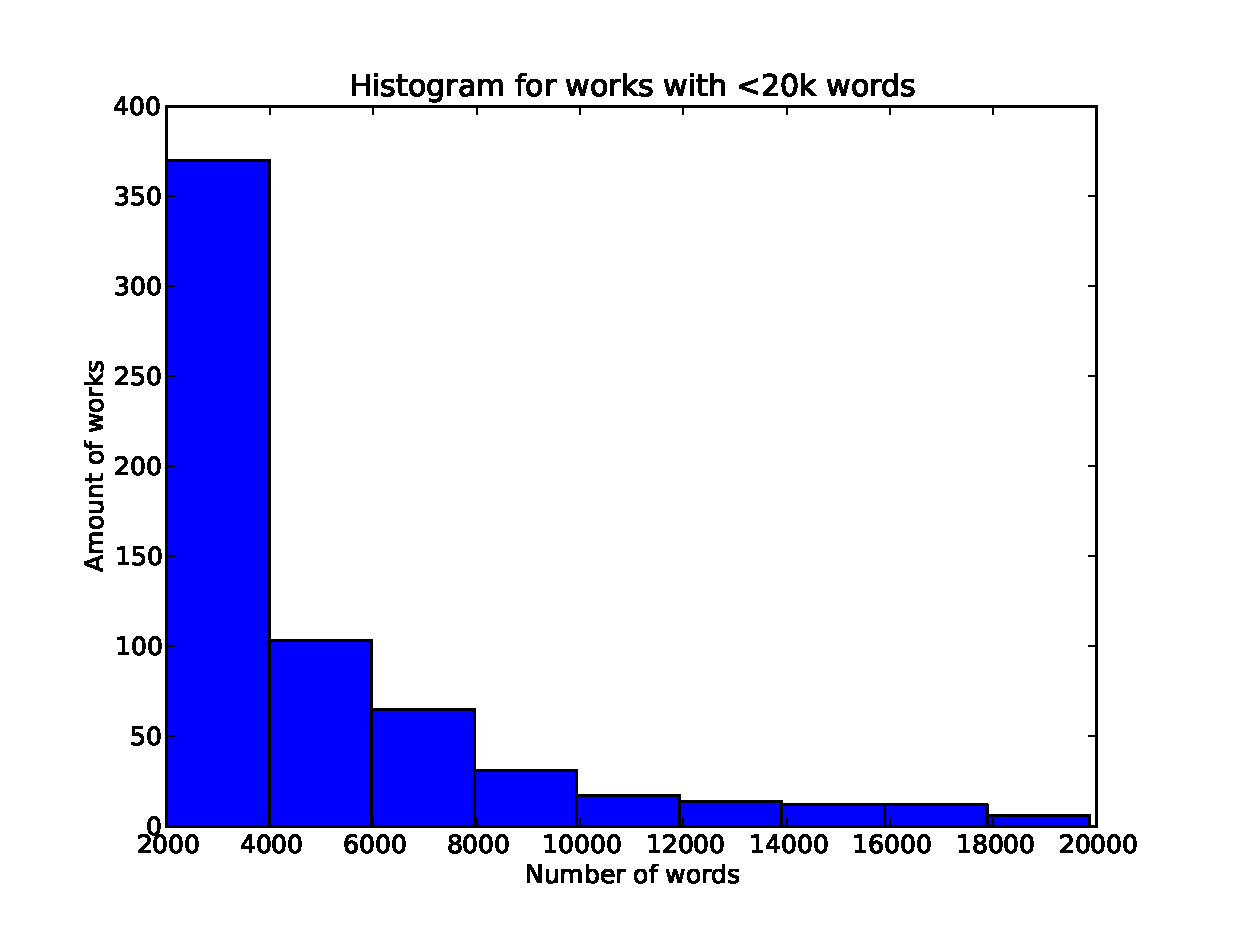
\includegraphics[width=.4\textwidth]{figures/hist_tokens_small_works.eps}}
\caption{Distribution of works with respect to size (small works)}\label{afoto}
\end{figure}


\begin{figure}
\centerline{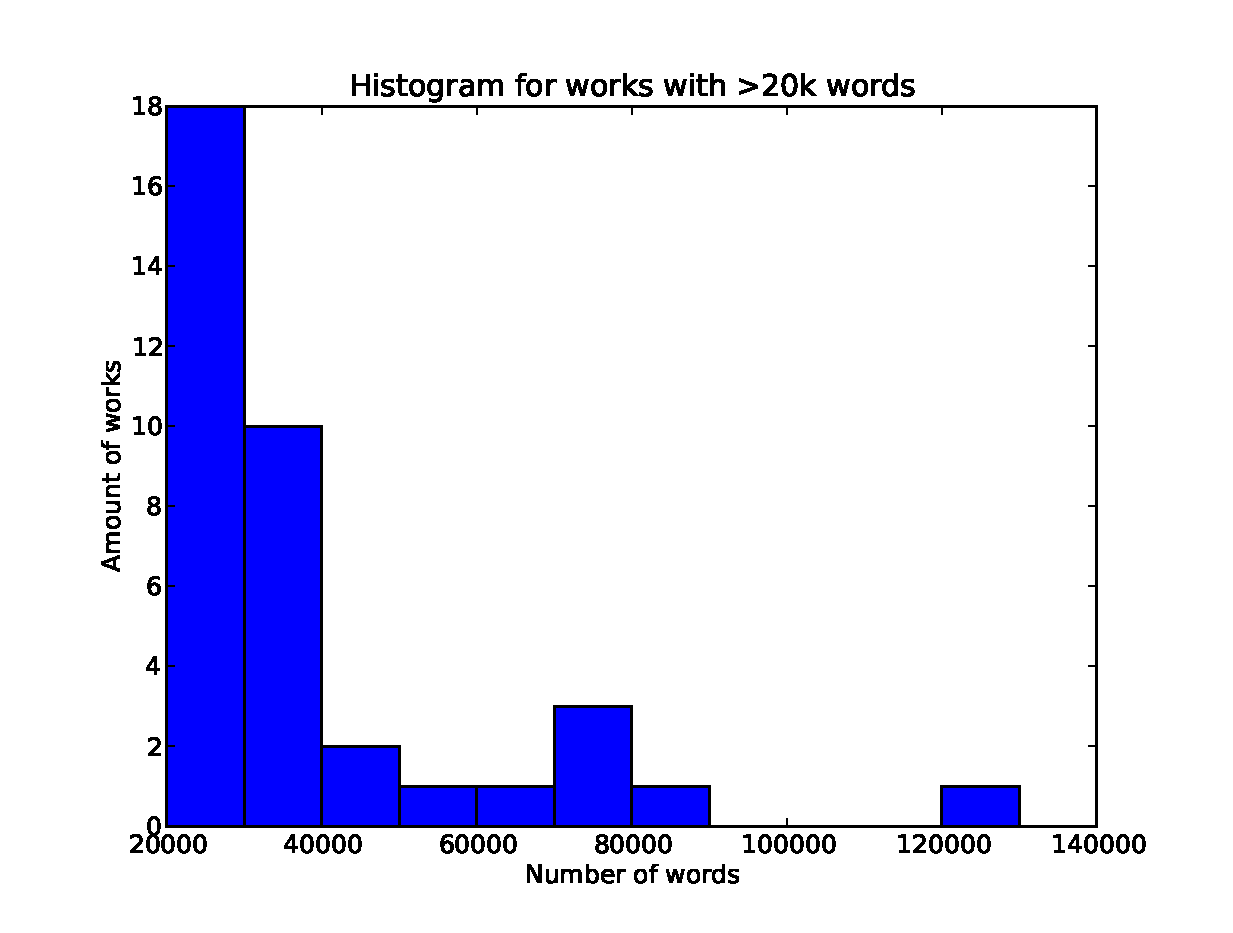
\includegraphics[width=.4\textwidth]{figures/hist_tokens_big_works.eps}}
\caption{Distribution of works with respect to size (big works)}\label{afoto}
\end{figure}


%*Números (obras totales obtenidas, promedio tokens)
\subsection{Information Value Framework}
\medskip
%
%*Aclarar settings de Zannette
%*Maximización, ventanas
%*Cálculo paralelo
%*Ajustes de parametros para que concuerden con los resultados de zanette
%*doc.top_words()
%  representación como set de palabras ponderadas por documento. 

\subsection{Wordnet analyzer}
Consideremos el siguiente problema:
\newline
¿Cómo calcular la similaridad o distancia de un documento a un cierto concepto? 
\newline
El enfoque que utilizamos en este trabajo es el de realizar una representación del documento como un conjunto de palabras, y en base a esto usar una noción topológica de similaridad/distancia. La proyección del documento al espacio de palabras la realizamos utilizando la t\'ecnica de Information Value reci\'en descripta.
En este espacio, utilizamos Wordnet para definir una noción de distancia entre el conjunto de palabras que representan al texto y diferentes conjuntos representando conceptos.
\newline
Para un documento dado, el módulo de information value genera una lista con lo $n$ términos más importantes y su iv. Estos valores se normalizan -dividiendo por la suma de los valores-, obteniendo así uno de los inputs del proceso siguiente. Recordemos, nuestro objetivo es asignar una distancia entre un documento y un concepto. Digamos, decidir cuán presente está o cuán importante es un concepto en un documento.
\newline
Wordnet es una base de datos de palabras, agrupadas en conjuntos de sinónimos (synsets), cada uno de los cuales posee una definición y diferentes relaciones semánticas con otros synsets (por ejemplo: hipernimia, hiponimia, meronimia, etc). Sobre estas relaciones semánticas es posible definir distintas métricas de distancia y similaridad entre synsets (Ver [1])
\newline
Utilizando las métricas disponibles en el módulo nltk de python para wordnet definimos la similaridad entre dos palabras como la máxima similaridad entre todos los synsets de ambas. (**NOTA Parametrizable: puede ser sólo el primer synset de ambos y puede no ser la máxima similaridad sino un promedio. También para algunas métricas quedan afuera los synsets que no son sustantivos). 
\begin{multline}
S_w(w_1, w_2) = max \{ S_s(s_1, s_2) \}: s_1 \in synsets(w_1),\\ s_2 \in synsets(w_2)
\end{multline}

Para path similarity vale que $0 \leq S_w \leq 1$. 

Sobre $S_w$ (de word similarity) definimos la similaridad de un documento a un término como:

\begin{equation}
S_{dw}(d, w) = sum \{ S_w(d_i, w) \times p(d_i)  \} 
\end{equation}

donde las tuplas $(d_i , p(d_i))$ representan las palabras más importantes del documento $d$, y sus respectivos pesos normalizados. Vale que $0 \leq p(d_i) \leq 1$ pues está normalizado.

Por ejemplo $S_{dw}$(“Estado y Revolución”, “guerra”) = NNN. $S_{dw}$ es una noción de cercanía entre un documento y una palabra.

Finalmente, definimos la noción de similaridad entre un año y una palabra como el promedio de las similaridades ($S_{dw}$) 
de los distintos documentos producidos durante ese año con la palabra en cuestión:
\begin{equation}
  S_{yw}(y, w) = mean \{ S_dw(y_i, w) \} : y_i \in docs(y) 
\end{equation}

Los resultados que presentaremos a continuaci\'on est\'an apoyados en distintas configuraciones de estas tres m\'etricas ($S_w$, $S_dw$ y $S_{yw}$).

% *WordnetAnalyzer
%   *Synset
%   *path, lch, wup
% *judge_word
% *judge_doc
% *judge_year
% Dado un conjunto de palabras, definimos la distancia de una palabra a este conjunto como 
% 

\section{Results}
\subsection{Resultados sobre obras}
* Tabla de top words de Estado y Revolución
\begin{center}
  \begin{tabular}{ | l | l | l |}
    \hline
    \multicolumn{3}{|c|}{Top words for `State and Revolution'} \\ \hline
    \# & Word & Information Value \\ \hline

    1 & kautsky & 0.10 \\ \hline
    2 &  marx & 0.09 \\ \hline
    3 &  revolution & 0.09 \\ \hline
    4 &  works & 0.06 \\ \hline 
    5 & engels & 0.06 \\ \hline
    6 &  society & 0.06 \\ \hline
    7 & power & 0.05 \\ \hline
    8 &  party & 0.04 \\ \hline
    9 &  social & 0.04 \\ \hline
    10 &  experience & 0.03 \\ \hline 
    11 & bernstein & 0.03 \\ \hline
    12 &  question & 0.03 \\ \hline 
    13 & equality & 0.03 \\ \hline
    14 &  phase & 0.03 \\ \hline
    15 & 1917 & 0.03 \\ \hline
    16 & commune & 0.03 \\ \hline
    17 & one & 0.03 \\ \hline
    18 & republic & 0.03 \\ \hline
    19 & class & 0.02 \\ \hline
    20 & law & 0.02 \\ \hline
  \end{tabular}
\end{center}


\begin{center}
  \begin{tabular}{ | r |l |}
    \hline
    \multicolumn{2}{|c|}{$S_{dw}($`State and Revolution'$, w)$} \\ \hline
      $w$ & $S_{dw}(d, w)$ \\ \hline
      revolution &  0.177  \\ \hline
      power &  0.169  \\ \hline
      state &  0.154  \\ \hline
      commune &  0.133  \\ \hline
      republic &  0.123  \\ \hline
      politics &  0.118  \\ \hline
      music &  0.114  \\ \hline
      war &  0.110  \\ \hline
      philosophy &  0.094  \\ \hline
      idealism &  0.084  \\ \hline
      chicken &  0.092  \\ \hline
      computer &  0.082  \\ \hline
      mosquito &  0.044  \\ \hline
      lion &  0.059  \\ \hline
      alcohol &  0.067  \\ \hline
      toilette &  0.069  \\ \hline
  \end{tabular}
\end{center}





* Distancia a algunos conceptos de estado y revolución

\subsection{Resultados sobre años}
*
* x = {años}, y = {concept value}

\section{Discussion}
* Zanette diferia en valores absolutos con los resultados nuestros. Moby Dick. 

\section{Acknowledgments}

\section{Literature cited}



\section{Analysis of almost sharp fronts}
We begin our analysis on almost sharp fronts for the
quasi-geostrophic equation recalling the notion of weak solution.

For these solutions we have the following


\subsection{Data Sources}
We are interested in studying the evolution of almost sharp fronts
for the QG equation. These are weak solutions of the equation with
large gradient ($\sim \displaystyle{ \inlinefrac{1}{\delta}}$, where $2
\delta$ is the thickness of the transition layer for $\theta$).



\begin{materials}
\section{Digital RNA SNP Analysis} A real-time PCR assay was designed
to amplify {\it PLAC4} mRNA, with the two SNP alleles being discriminated
by TaqMan probes. {\it PLAC4} mRNA concentrations were quantified in
extracted RNA samples followed by dilutions to approximately one target
template molecule of either type (i.e., either allele) per well.
Details are given in the {\it SI Materials and Methods}.

\section{Digital RCD Analysis} Extracted DNA was quantified by
spectrophotometry (NanoDrop Technologies, Wilmington, DE) and diluted to a
concentration of 
approximately one target template from either chr21 or ch1 per well.
\end{materials}

\appendix[Entropy of a word in a text]

Let's recall from \cite{DARWIN} and \cite{ENTROPIC} the concept of information value of a word. 
Let $T$ be a text, which has been split into $P$ pieces $T_1, T_2, \dots, T_P$, $w$ be a word in $T$,
and $f_i$ the frequency of appearance of $w$ in $T_i$.

For each part $1 \leq i \leq P$, we could define:

\begin{equation}
  p_i = \frac{f_i}{\Sigma_{j=1}^{P}f_i}
\end{equation}

This quantity stands for probability of finding $w$ in $T_i$, given that it is present in the text. So, 
we define the Shannon information entropy of $w$ in $T$ as

\begin{equation}
  S = -\frac{1}{ln P}\sum_{i=1}^{P}p_i ln p_i
\end{equation}


\appendix[Estimating the Spectral Norm of a Matrix]
In this appendix we describe a method for the estimation of the spectral norm
of matrix $A$. The method does not require access to the individual
entries of $A$; it requires only applications of $A$ and $A$* to vectors.
It is a version of the classical power method. Its probabilistic
analysis summarized below was introduced fairly recently in refs. 13
and 14. This appendix is included here for completeness.


\appendix
This is an example of an appendix without a title.

\begin{acknowledgments}
This work was partially supported by 
Spanish Ministry of Science and Technology Grant BFM2002-02042 (to D.C. and
J.L.R.) and by National Science Foundation Grand DMS-0245242 (to C.F.).
\end{acknowledgments}



\begin{thebibliography}{10}
\bibitem{DARWIN}
M.A. Montemurro and D. H. Zanette, {\em The statistics of meaning: Darwin, Gibbon and Moby Dick}, Significance, Dec. 2009, 165-169.
\bibitem{ENTROPIC}
M.A. Montemurro and D. H. Zanette, {\em Entropic analysis of the role of words in literary texts}, Adv. Complex Systems 5, September 27th 2001
\end{thebibliography}
\end{article}


\begin{table}[h]
\caption{Repeat length of longer allele by age of onset class.
This is what happens when the text continues.}
\begin{tabular}{@{\vrule height 10.5pt depth4pt  width0pt}lrcccc}
&\multicolumn5c{Repeat length}\\
\noalign{\vskip-11pt}
Age of onset,\\
\cline{2-6}
\vrule depth 6pt width 0pt years&\multicolumn1c{\it n}&Mean&SD&Range&Median\\
\hline
Juvenile, 2$-$20&40&60.15& 9.32&43$-$86&60\\
Typical, 21$-$50&377&45.72&2.97&40$-$58&45\\
Late, $>$50&26&41.85&1.56&40$-$45&42\tablenote{The no. of wells for all samples was 384. Genotypes were
determined by mass spectrometric assay. The $m_t$ value indicates the
average number of wells positive for the over represented allele.}
\\
\hline
\end{tabular}
\end{table}


\begin{table*}[ht]
\caption{Summary of the experimental results}
\begin{tabular*}{\hsize}
{@{\extracolsep{\fill}}rrrrrrrrrrrrr}
\multicolumn{3}{l}{Parameters}&
\multicolumn{5}{c}{Averaged Results}&
\multicolumn{5}{c}{Comparisons}\cr
\hline
\multicolumn1c{$n$}&\multicolumn1c{$S^*_{MAX}$}&
\multicolumn1c{$t_1$}&\multicolumn1c{\ $r_1$}&
\multicolumn1c{\ $m_1$}&\multicolumn1c{$t_2$}&
\multicolumn1c{$r_2$}&\multicolumn1c{$m_2$}
&\multicolumn1c{$t_{lb}$}&\multicolumn1c{\ \ $t_1/t_2$}&
$r_1/r_2$&$m_1/m_2$&
$t_1/t_{lb}$\cr
\hline
10\tablenote{Stanford Synchrotron Radiation Laboratory (Stanford University,
Stanford, CA)}&1\quad &4&.0007&4&4&.0020&4&4&1.000&.333&1.000&1.000\cr
10\tablenote{$R_{\rm FREE}=R$ factor for the $\sim 5$\% of the randomly
chosen unique ref\/lections not used in the ref\/inement.}&5\quad &50&.0008&8&50&.0020&12&49&.999&.417&.698&1.020\cr
100\tablenote{Calculated for all observed data}&20\quad &2840975&.0423&95&2871117&.1083&521&---&
.990&.390&.182&---\ \ \cr
\hline
\end{tabular*}
\end{table*}






\end{document}


